\section{The Quantum Half Adder}
In this section we are going to construct, using the Qiskit SDK, a quantum circuit that implements the classic Half-Adder circuit.
First we shall consider the classic circuit diagram of the Half-Adder circuit from Chapter 2.

\subsection{Analysing the diagram and logic of the Quantum Half-Adder}

\begin{figure}[ht]
    \centering
    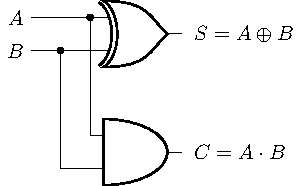
\includegraphics{images/5_Implementation/classical_halfadder_diagram.pdf}
    \caption{The classical Half-Adder circuit diagram}
\end{figure}

The circuit takes two 1-bit inputs, $A$ and $B$ and produces two 1-bit outputs $S$ (the sum, $A + B$) and $C$ (the possible carry of $S$).
As we can see from the diagram, to compute the sum of the inputs we have to apply an XOR gate on the inputs. As for the carry, we apply the
AND gate. From this simple analysis we can produce the truth table of this circuit to better construct its quantum-counterpart.

\begin{table}[ht]
    \centering
    \begin{tabular}{c c|c c}
        $A$ & $B$ & $S = A \oplus B$ & $C = A \cdot B$ \\
        \hline
        $0$ & $0$ & $0$ & $0$ \\
        $0$ & $1$ & $1$ & $0$ \\
        $1$ & $0$ & $1$ & $0$ \\
        $1$ & $1$ & $0$ & $1$ \\
    \end{tabular}
    \caption{The truth table of the classical Half-Adder circuit}
\end{table}

Now the construction of the quantum Half-Adder is matter of matching the boolean functions, the XOR and AND function to be exact, to the
appropriate quantum gates.

Let $A$ and $B$ be two 1-qubit inputs. The XOR boolean function maps directly with the Feynman gate (or controlled-NOT/CNOT gate). We can deduce that
from comparing the two gates truth table.

\begin{table}[ht]
    \centering
    \begin{subtable}[h]{0.45\textwidth}
        \centering
        \begin{tabular}{cc|c}
            $\ket{A}$ & $\ket{B}$ & $\ket{B}'=\ket{A \oplus B}$ \\
            \hline
            $0$ & $0$ & $0$ \\
            $0$ & $1$ & $1$ \\
            $1$ & $0$ & $1$ \\
            $1$ & $1$ & $0$ \\
        \end{tabular}
        \caption{CNOT's truth table}
    \end{subtable}
    \begin{subtable}[h]{0.45\textwidth}
        \centering
        \begin{tabular}{cc|c}
            $A$ & $B$ & $A \oplus B$ \\
            \hline
            $0$ & $0$ & $0$ \\
            $0$ & $1$ & $1$ \\
            $1$ & $0$ & $1$ \\
            $1$ & $1$ & $0$ \\
        \end{tabular}
        \caption{XOR's truth table}
    \end{subtable}
    \caption{The truth tables of the CNOT (a) and XOR (b) gates side-by-side}
\end{table}

We omitted the third column from table (a) to better emphasize the similarities of the two gates.

The AND boolean function cannot be mapped directly to any quantum gate/operation because it is not reversible. This does not mean that it is
impossible to construct the same functionality using quantum gates. We shall borrow a \say{garbage} qubit $\ket{O} = 0$ to simulate the boolean AND function.
By applying the Toffoli gate with control qubits $\ket{A}$, $\ket{B}$ and the borrowed qubit $\ket{O}$, as the target, we simulate the AND functionality
directly.

\begin{figure}[ht]
    \centering
    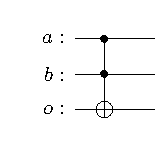
\includegraphics{images/5_Implementation/toffoli_gate_diagram.pdf}
    \caption{The Toffoli gate diagram}
\end{figure}

At the end of the computation, $\ket{O}$ will store the conjunction of $\ket{A}$ and $\ket{B}$. This can be seen more clearly from the side-by-side
view of the truth tables of the two gates.

\begin{table}[ht]
    \centering
    \begin{subtable}[h]{0.45\textwidth}
        \centering
        \begin{tabular}{ccc|c}
            $\ket{A}$ & $\ket{B}$ & $\ket{O}$ & $\ket{O}'=\ket{A \cdot B}$ \\
            \hline
            $0$ & $0$ & $0$ & $0$ \\
            $0$ & $1$ & $0$ & $0$ \\
            $1$ & $0$ & $0$ & $0$ \\
            $1$ & $1$ & $0$ & $1$ \\
        \end{tabular}
        \caption{CCNOT's truth table}
    \end{subtable}
    \begin{subtable}[h]{0.45\textwidth}
        \centering
        \begin{tabular}{cc|c}
            $A$ & $B$ & $A \cdot B$ \\
            \hline
            $0$ & $0$ & $0$ \\
            $0$ & $1$ & $1$ \\
            $1$ & $0$ & $1$ \\
            $1$ & $1$ & $0$ \\
        \end{tabular}
        \caption{AND's truth table}
    \end{subtable}
    \caption{The truth tables of the Toffoli/CCNOT (a) and AND (b) gates side-by-side}
\end{table}

The complete circuit has to be constructed with caution because if we apply the CNOT gate first, we inevitably change the state of $\ket{B}$. With this
knowledge at hand we have to apply the CCNOT gate as the first computational step and later the CNOT gate.

\begin{figure}[ht]
    \centering
    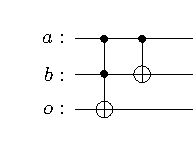
\includegraphics{images/5_Implementation/half_adder.pdf}
    \caption{The quantum Half-Adder circuit with slices that indicate each computational step}
\end{figure}

We are going to enumerate over each computational step:
\begin{enumerate}
    \item $\ket{O'} = CCNOT\ket{A}\otimes\ket{B}\otimes\ket{O} = CCNOT\ket{A,B,O} = \ket{A \oplus B}$
    \item $\ket{B'} = CNOT\ket{A}\otimes\ket{B} = \ket{A \cdot B}$
\end{enumerate}

\begin{table}[ht]
    \centering
    \begin{tabular}{ccc|ccc}
        $\ket{A}$ & $\ket{B}$ & $\ket{O}$ & $\ket{A'} = \ket{A}$ & $\ket{B'} = \ket{C}$ & $\ket{O'} = \ket{S}$ \\
        \hline
        $0$ & $0$ & $0$ & $0$ & $0$ & $0$ \\
        $0$ & $1$ & $0$ & $0$ & $0$ & $1$ \\
        $1$ & $0$ & $0$ & $1$ & $0$ & $1$ \\
        $1$ & $1$ & $0$ & $1$ & $1$ & $0$ \\
    \end{tabular}
    \caption{The truth table of the quantum Half-Adder circuit}
\end{table}

As we can see $\ket{B'}$ stores the carry of $A$ and $B$ and $\ket{O'}$ stores the sum of $A$ and $B$.

\subsection{The Python3 implementation}

First we need to import some useful classes from the Qiskit library. \mintinline{python3}{QuantumCircuit} and \\
\mintinline{python3}{QuantumRegister} will be used to create the Half-Adder circuit.

\begin{listing}[ht]
    \centering
    \begin{minted}{python3}
        from qiskit import QuantumCircuit, QuantumRegister
    \end{minted}
    \caption{The initial imports for the quantum Half-Adder circuit}
\end{listing}


After importing the initial classes we instantiate three object $A, B$ and $O$, which are all \\\mintinline{python3}|QuantumRegister|'s and
one object which is a \mintinline{python3}|QuantumCircuit|.

\begin{listing}[ht]
    \centering
    \begin{minted}{python3}
        a = QuantumRegister(1, name="A")
        b = QuantumRegister(1, name="B")
        o = QuantumRegister(1, name="O")
        circuit = QuantumCircuit(a, b, o)
    \end{minted}
    \caption{Instantiating the circuit object of the quantum Half-Adder circuit}
\end{listing}

We can now apply all the necessary operations to compute the sum and the carry of $A$ and $B$. First we apply the CCNOT gate to the circuit,
with control qubits $A$, $B$ and as the target qubit $O$. This can be done by calling the \mintinline{python3}|circuit.ccx()| method of the
\mintinline{python3}|QuantumCircuit| class.

Lastly we apply the CNOT gate, with control qubit $A$ and target qubit $B$. This can be done by calling the \mintinline{python3}|circuit.cx()|
method of the \mintinline{python3}|QuantumCircuit| class.

Putting it all together, we can implement the computational steps from Figure 5.3.

\begin{listing}[ht]
    \centering
    \begin{minted}{python3}
        circuit.ccx(a, b, o)
        circuit.cx(a, b)
    \end{minted}
    \caption{The computational steps of the Half-Adder in Python3}
\end{listing}